\documentclass[11pt, a4paper, twoside]{article}
\usepackage{graphicx}
\usepackage{amsmath}
\usepackage[margin=0.8in]{geometry}
\usepackage{listings}
\usepackage{float}
\usepackage{fancyhdr}
\usepackage{indentfirst}
\usepackage[inline]{enumitem}
\usepackage{xcolor}
\usepackage{minted}
\usemintedstyle{vs}
\usepackage[belowskip=0pt,aboveskip=0pt,font=small,labelfont=small]{caption}
\captionsetup{width=0.9\linewidth}
\setlength\intextsep{0pt}

\setlist[itemize]{noitemsep, topsep=0pt}
\fancyhead[RO,LE]{EE2703: Assignment 4}
\fancyhead[LO,RE]{Akilesh Kannan}
\cfoot{\thepage}

\title{EE2703: Assignment 4}
\author{Akilesh Kannan(EE18B122)}
\date{\today}

\pagestyle{fancy}

\begin{document}
    \maketitle
    \section{Abstract}
         In this assignment, I look at approximating a few functions using the Fourier series. I will employ two methods to find the Fourier approximation of $e^x$ and $cos(cos(x))$: \begin{enumerate}[label=\textbf{(\alph*)}, noitemsep, topsep=0pt]
            \item Direct Integration
            \item Least Squares Method
        \end{enumerate}

        I shall also compare the Fourier coefficients I have got in the two methods and see how close the Fourier approximation is to the true function.

    \section{Theory}
        \textit{Any periodic function can be expressed as a linear combination of various sinusoids.} This is the underlying principle of the Fourier Approximation. We can also approximate any function in the domain [0,2$\pi$) by slightly `tweaking' the mathematics of the Fourier series by extending copies of the function between [0,2$\pi$) till infinity, thus creating a periodic function.

        For a function $f(x)$, it's Fourier series is given as:
        \begin{equation}
            f(x) = a_0 + \sum_{k=1}^{\infty}a_kcos(kx) + b_ksin(kx)
        \end{equation}
        where,
        \begin{equation}
            a_0 = \frac{1}{2\pi}\int_{0}^{2\pi}f(x)dx
        \end{equation}
        \begin{equation}
            \begin{split}
                a_k = \frac{1}{\pi}\int_{0}^{2\pi}f(x)cos(kx)dx\\
                b_k = \frac{1}{\pi}\int_{0}^{2\pi}f(x)sin(kx)dx
            \end{split}
        \end{equation}

        The above equations describe the \textit{Direct Integration} method of finding the Fourier approximation. We shall also use the \textit{Least Squares} method we learnt in the last assignment to find the Fourier approximation.

    \section{Tasks}
        I shall now walk through the tasks that were asked to be performed and also include the necessary portions of the code and any associated plots.
        \subsection{Question 1}
            \begin{itemize}[label=-]
                \item Define Python functions for the two functions $e^x$ and $cos(cos(x))$ which return a vector (or scalar) value.
                \item Plot the functions over the interval $[-2\pi,4\pi)$.
                \item Discuss periodicity of both functions.
                \item Plot the expected functions from Fourier series.
            \end{itemize}
            \subsubsection{Code}
                \inputminted[linenos, breaklines]{python}{Code/q1.py}
            \subsubsection{Plots}
                \begin{figure}[H]
                    \centering
                    \setlength\tabcolsep{2pt}
                    \begin{tabular}{cc}
                        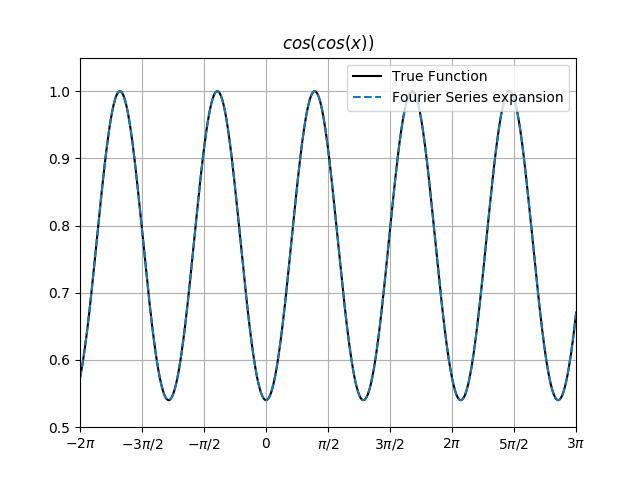
\includegraphics[scale=0.5]{Plots/Figure 1.png} &
                        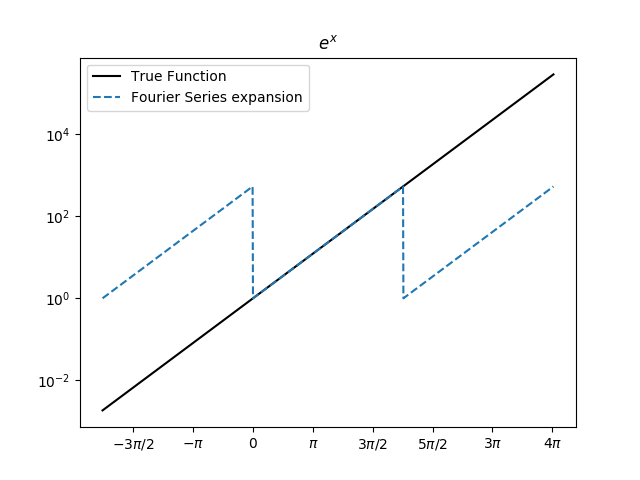
\includegraphics[scale=0.5]{Plots/Figure 2.png}\\
                    \end{tabular}
                \end{figure}
            \subsubsection{Discussions}
                \begin{enumerate}
                    \item From the above plots, you can easily see that while $cos(cos(x))$ is periodic with period $2\pi$, the latter, $e^x$ isn't periodic and rises monotonically.
                    \item From the Fourier series, we expect that the Fourier approximation of the function would be repetitions of the function between $[0, 2\pi)$. We can thus say that the Fourier approximation of the function $f(x)$ is $f(x\mod2\pi)$\footnote{It is actually $f(x\mod p)$, where $p$ the minimum among the period of the periodic function and $2\pi$.}.
                \end{enumerate}
        \subsection{Question 2}
            \begin{itemize}[label=-]
                \item Obtain the first 51 coefficients i.e., $a_0$, $a_1$, $b_1$,\ldots for $e^x$ and $cos(cos(x))$ using \texttt{quad} function.
                \item Calculate the function using those coefficients and compare with original functions graphically.
            \end{itemize}
            \subsubsection{Code}
                \inputminted[linenos, breaklines]{python}{Code/q2.py}
            \subsubsection{Discussions}
                The function \mintinline{python}{calc51FourierCoeffs(f)} takes in the name of a function as argument and returns the first 51 coefficients of the function \texttt{f}, in order, as an array. One advantage of hard-coding the number 51 is that it becomes faster, while the hard-coding makes it difficult for the function to be generalised.

        \subsection{Question 3}
            \begin{itemize}
                \item[-] Two  different  plots  for  each  function  using  \texttt{semilogy}  and  \texttt{loglog} and plot the magnitude of the coefficients versus n.
            \end{itemize}
            \subsubsection{Code}
                \inputminted[linenos, breaklines]{python}{Code/q3.py}
            \subsubsection{Plots}
                \begin{figure}[H]
                    \centering
                    \setlength\tabcolsep{2pt}
                    \begin{tabular}{cc}
                       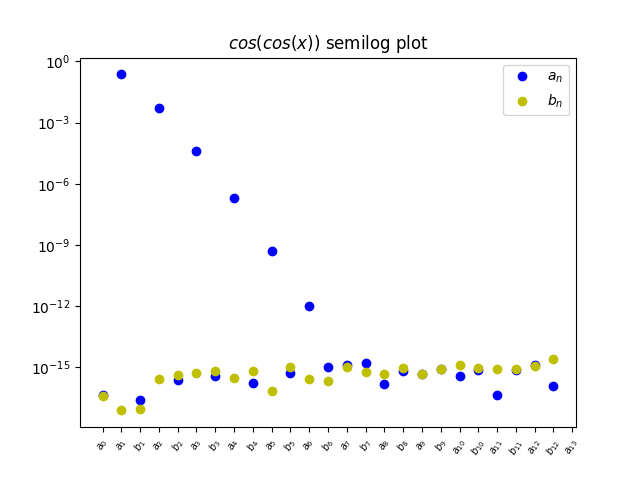
\includegraphics[scale=0.5]{Plots/Figure 3.png} &
                       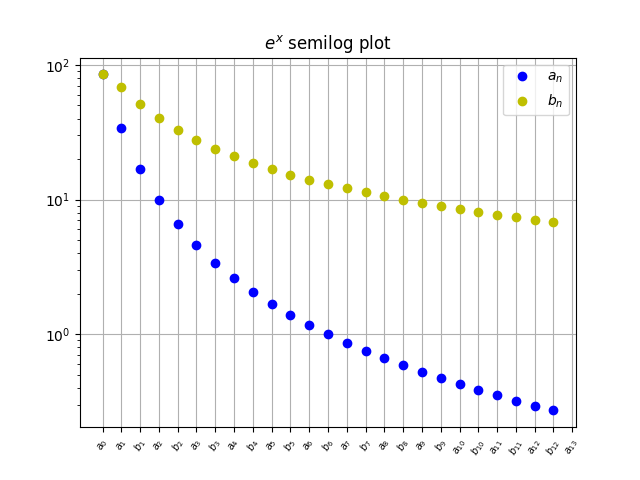
\includegraphics[scale=0.5]{Plots/Figure 4.png}\\
                       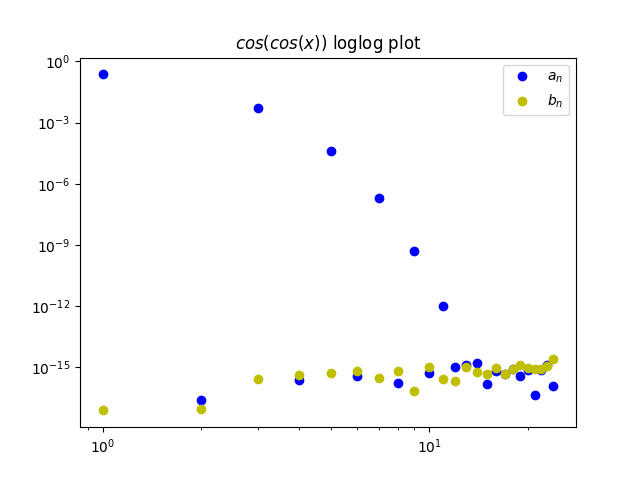
\includegraphics[scale=0.5]{Plots/Figure 5.png} &
                       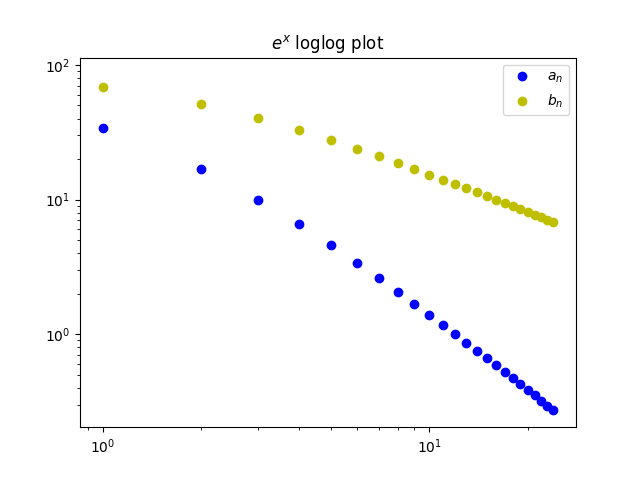
\includegraphics[scale=0.5]{Plots/Figure 6.png}\\
                    \end{tabular}
                \end{figure}
            \subsubsection{Discussions}
                \begin{enumerate}[label=(\alph*)]
                    \item As we can see from the above plots, almost all $b_n$ coefficients are very close to 0 for $cos(cos(x))$. This is expected - we find by hand integration that the $b_n$ coefficients are 0 (due to the odd nature of the integrand between $[-\pi,\pi)$.

                    It does not become exactly zero due to approximations used in the implementation of the \texttt{quad} function.

                    \item Rate of decay of Fourier coefficients is determined by how smooth the  function is - if a function is infinitely differentiable then its Fourier coefficients decay very fast. But if the $k^{th}$ derivative of the function $f$, denoted by $f^{(k)}$, is discontinuous, then the rate of decay of the Fourier coefficients is only $\frac{1}{n^k}$.

                    Since $cos(cos(x))$ is an infinitely differentiable function, it's Fourier coefficients decay very fast, while that of $e^x$ decay very slowly due to the discontinuity in the Fourier approximation of the function at $2n\pi$.

                    \item
                \end{enumerate}
        \subsection{Questions 4 \& 5}
            \begin{itemize}
                \item[-] Use a \textit{Least Squares} approach to find the Fourier coefficients of the functions, using \texttt{scipy.linalg.lstsq}.
                \item[-] Build the coefficient matrix $A$ and the constant matrix $b$.
            \end{itemize}

            \subsubsection{Code}
                \inputminted[linenos, breaklines]{python}{Code/q4.py}
        \subsection{Question 6}
            \begin{itemize}
                \item[-] Compare the coefficients obtained through the \textit{least squares method} and the \textit{direct integration} method.
                \item[-] Find the maximum deviation between the coefficients obtained in the two methods.
            \end{itemize}
            \subsubsection{Code}
                \inputminted[linenos, breaklines]{python}{Code/q6.py}
            \subsubsection{Plots}
                \begin{figure}[H]
                    \begin{tabular}{cc}
                        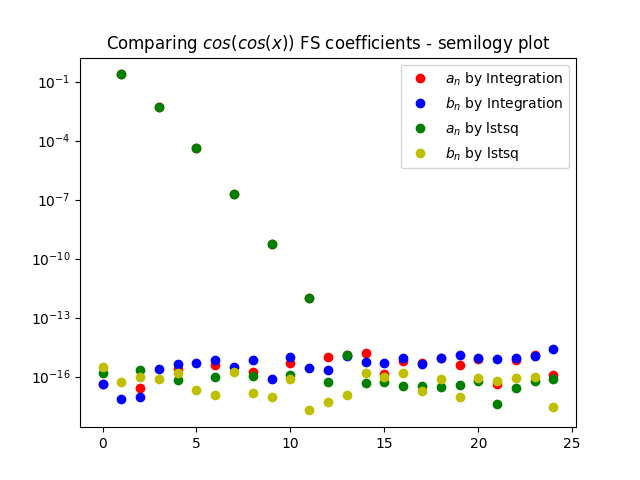
\includegraphics[scale=0.5]{Plots/Figure 3.1.png} &
                        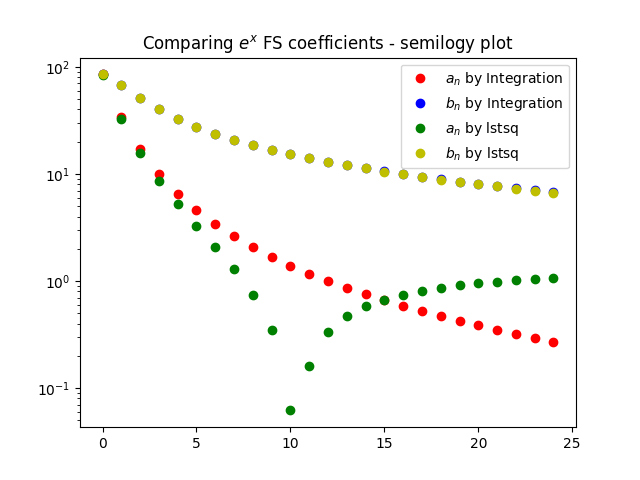
\includegraphics[scale=0.5]{Plots/Figure 4.1.png}\\
                        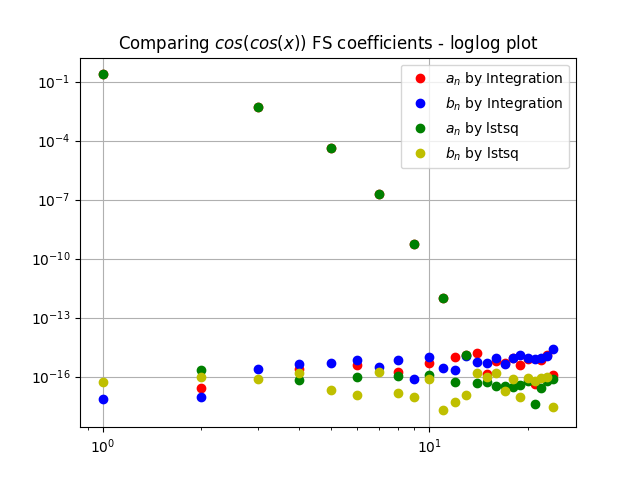
\includegraphics[scale=0.5]{Plots/Figure 5.1.png} &
                        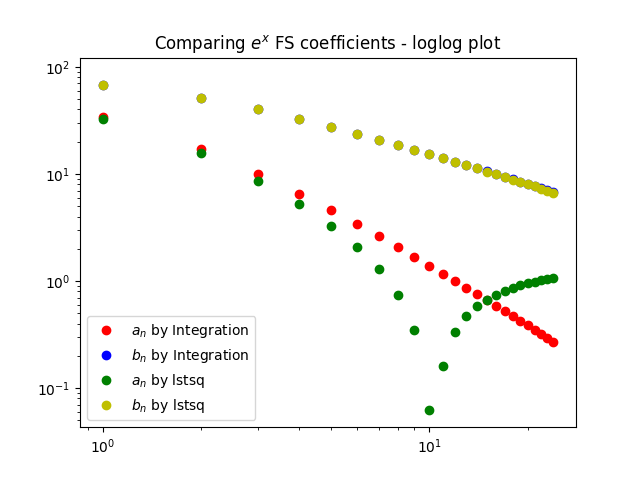
\includegraphics[scale=0.5]{Plots/Figure 6.1.png}\\
                    \end{tabular}
                \end{figure}
            \subsubsection{Discussion}
        \subsection{Question 7}
            \begin{itemize}
                \item[-] Computing $A\cdot c$ from the estimated values of $c$ by \textit{Least Squares Method} and plotting them.
            \end{itemize}
            \subsubsection{Code}
                \inputminted[linenos, breaklines]{python}{Code/q7.py}
            \subsubsection{Plots}
                \begin{figure}[H]
                    \begin{tabular}{cc}
                        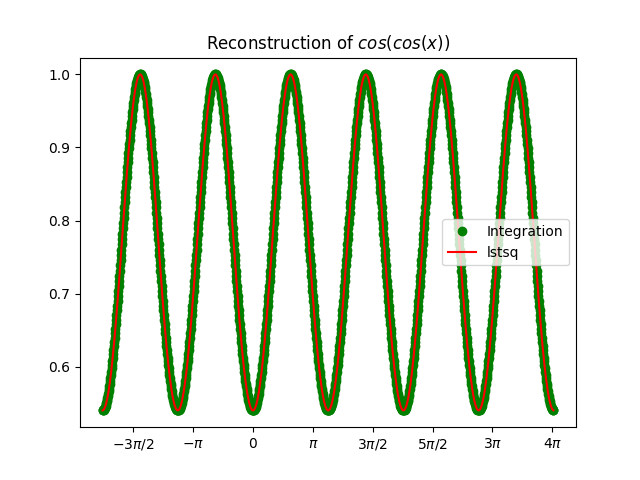
\includegraphics[scale=0.5]{Plots/Figure 7.png} &
                        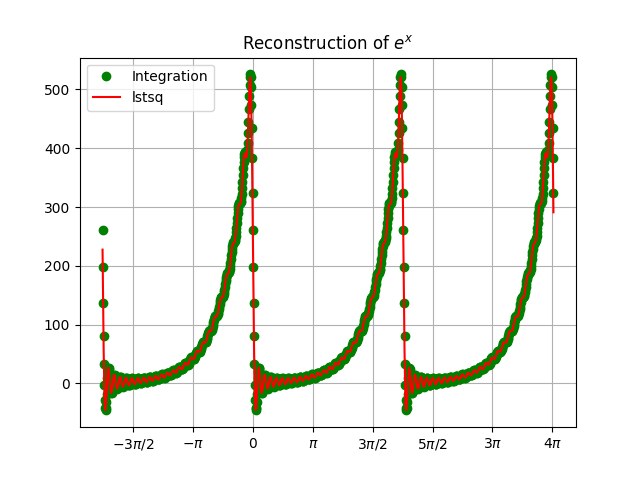
\includegraphics[scale=0.5]{Plots/Figure 8.png}\\
                    \end{tabular}
                \end{figure}
            \subsubsection{Discussion}

            \begin{itemize}[label=-]

            \item
              As we observe that there is a significant deviation for \(e^{x}\) as
              it has discontinuities at \(2n\pi\) which can be observed in the figure,
              and so there will be \textbf{Gibbs phenomenon} i.e, there will be
              oscillations around the discontinuity points and their ripple
              amplitude will decrease as we go close to discontinuity. In this case
              it is at \(2\pi\) for \(e^{x}\).
            \item
              As we observe that ripples are high initially and reduces and
              oscillate with more frequency as we go towards \(2\pi\). This
              phenomenon is called \textbf{Gibbs Phenomenon}
            \item
              Due to this, the original function and one which is reconstructed using
              least squares will not fit exactly.
            \item
              And as we know that Fourier series is used to define periodic signals
              in frequency domain and \(e^{x}\) is a aperiodic signal so you can't
              define an aperiodic signal on an interval of finite length (if you
              try, you'll lose information about the signal), so one must use the
              Fourier transform for such a signal.
            \item
              That is why there are significant deviations for \(e^{x}\) from original
              function.
            \item
              For\(\cos(\cos(x))\) the curves fit almost perfectly because
              the function itself is a periodic function and it is a continuous
              function everywhere, so we get very negligible deviation and
              able to reconstruct the signal with just the Fourier coefficients.
            \end{itemize}
    \section{Conclusion}
    We see that the Fourier estimation of \(e^x\) does not match
significantly with the function close to \(0\), but matches near
perfectly in the case of \(\cos(\cos(x))\). This is due to the
presence of a discontinuity at \(x=0\) for the periodic extension of
\(e^x\). This discontinuity leads to non-uniform convergence of the
Fourier series, with different rates for both the functions.

The difference in the rates of convergence leads to the \textbf{Gibb's
phenomenon}, which is the ringing observed at discontinuities in the
Fourier estimation of a discontinuous function.
This explains the mismatch in the Fourier approximation for \(e^x\).

Thus we can conclude that the Fourier Series Approximation Method works extremely well
for smooth periodic functions, but gives bad results for discontinuous periodic functions
\end{document}
\end{document}
